\section{Additional visualizations}

\begin{figure}[h]
\begin{subfigure}[t]{0.3\textwidth}
    \centering
    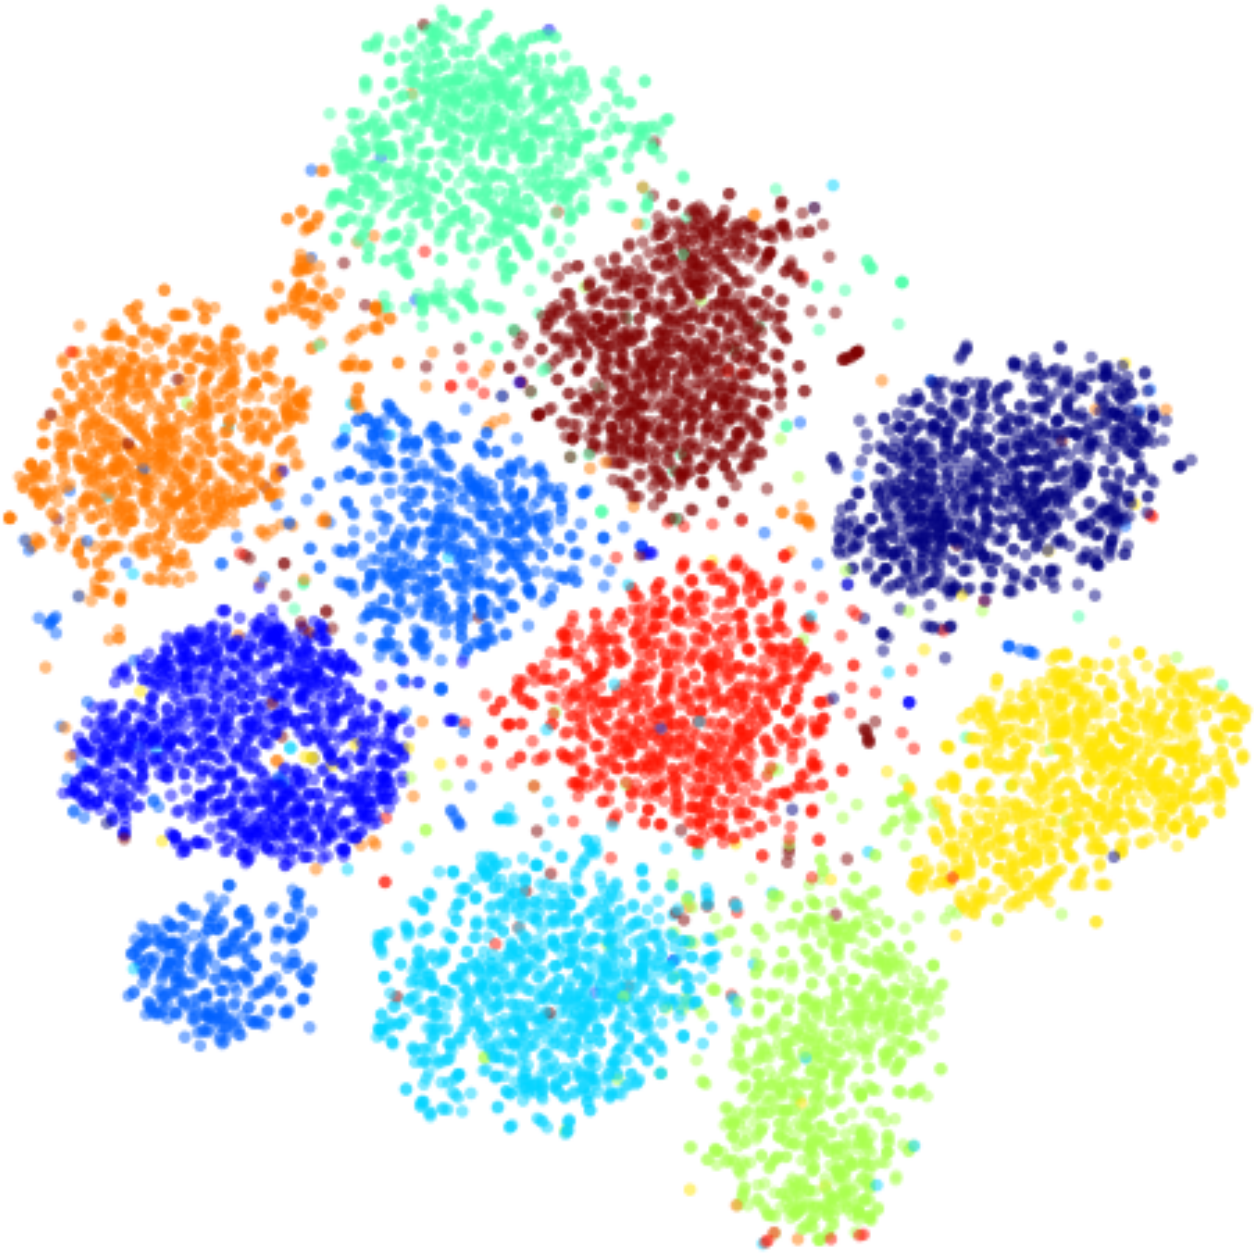
\includegraphics[width=\textwidth]{img/loracs/mnist/tsne/mnist2-tsne-normal.png}
    \caption{Normal prior}
\end{subfigure}
\begin{subfigure}[t]{0.3\textwidth}
    \centering
    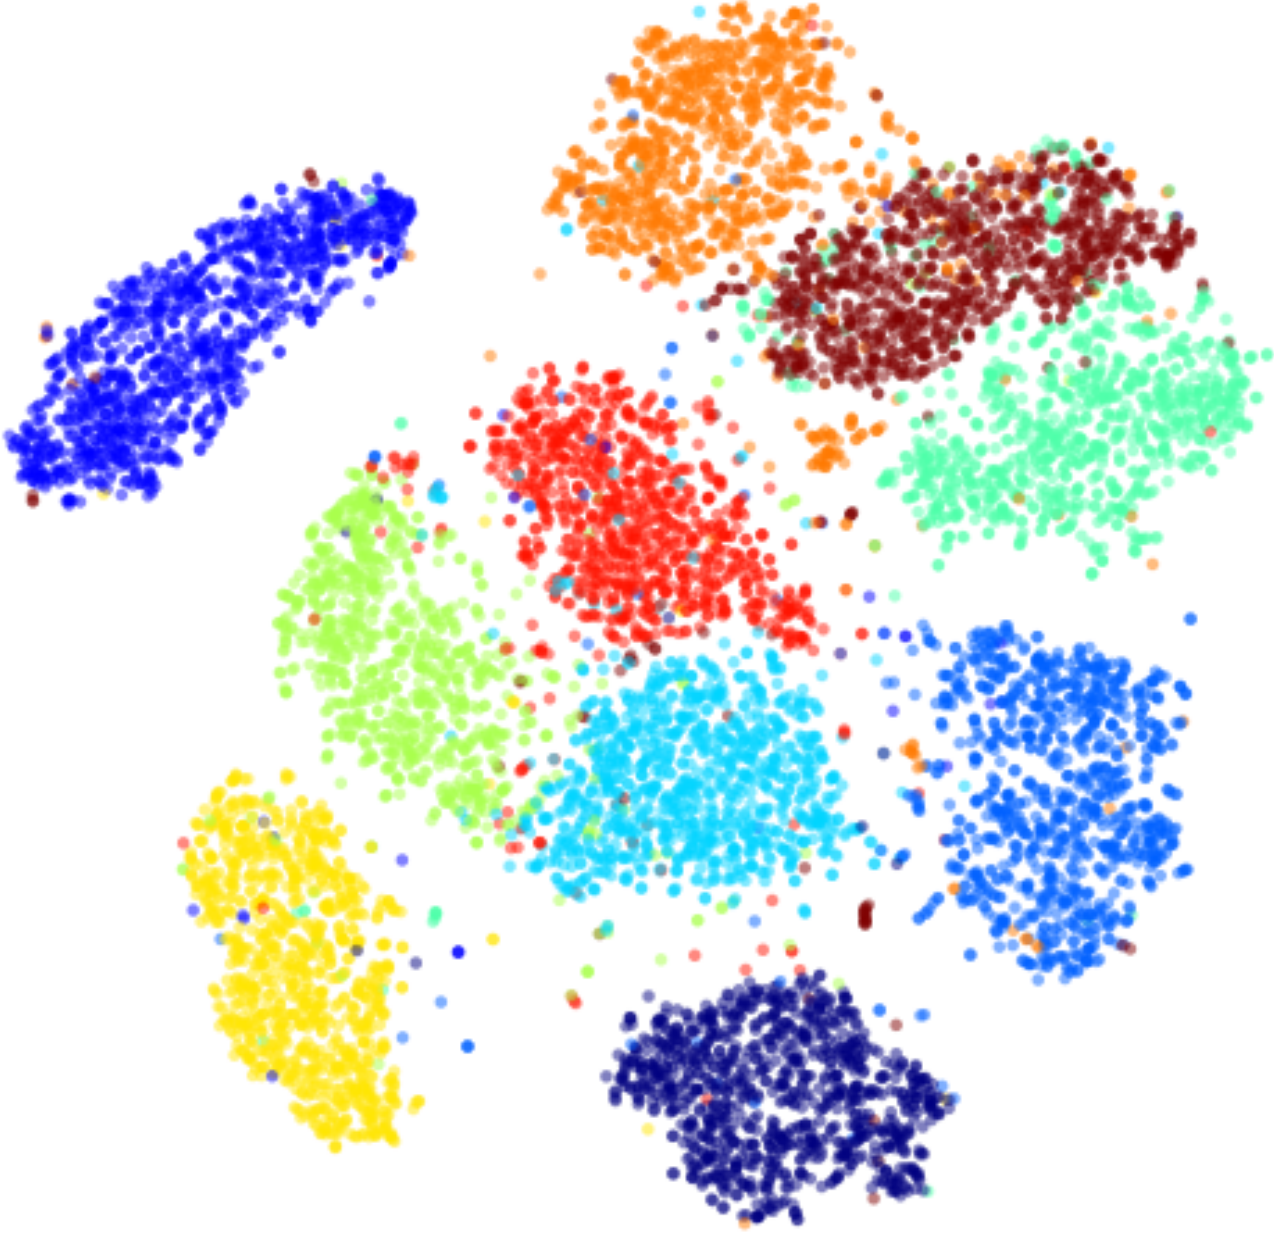
\includegraphics[width=\textwidth]{img/loracs/mnist/tsne/mnist2-tsne-noprior.png}
    \caption{No prior}
\end{subfigure}
\begin{subfigure}[t]{0.3\textwidth}
    \centering
    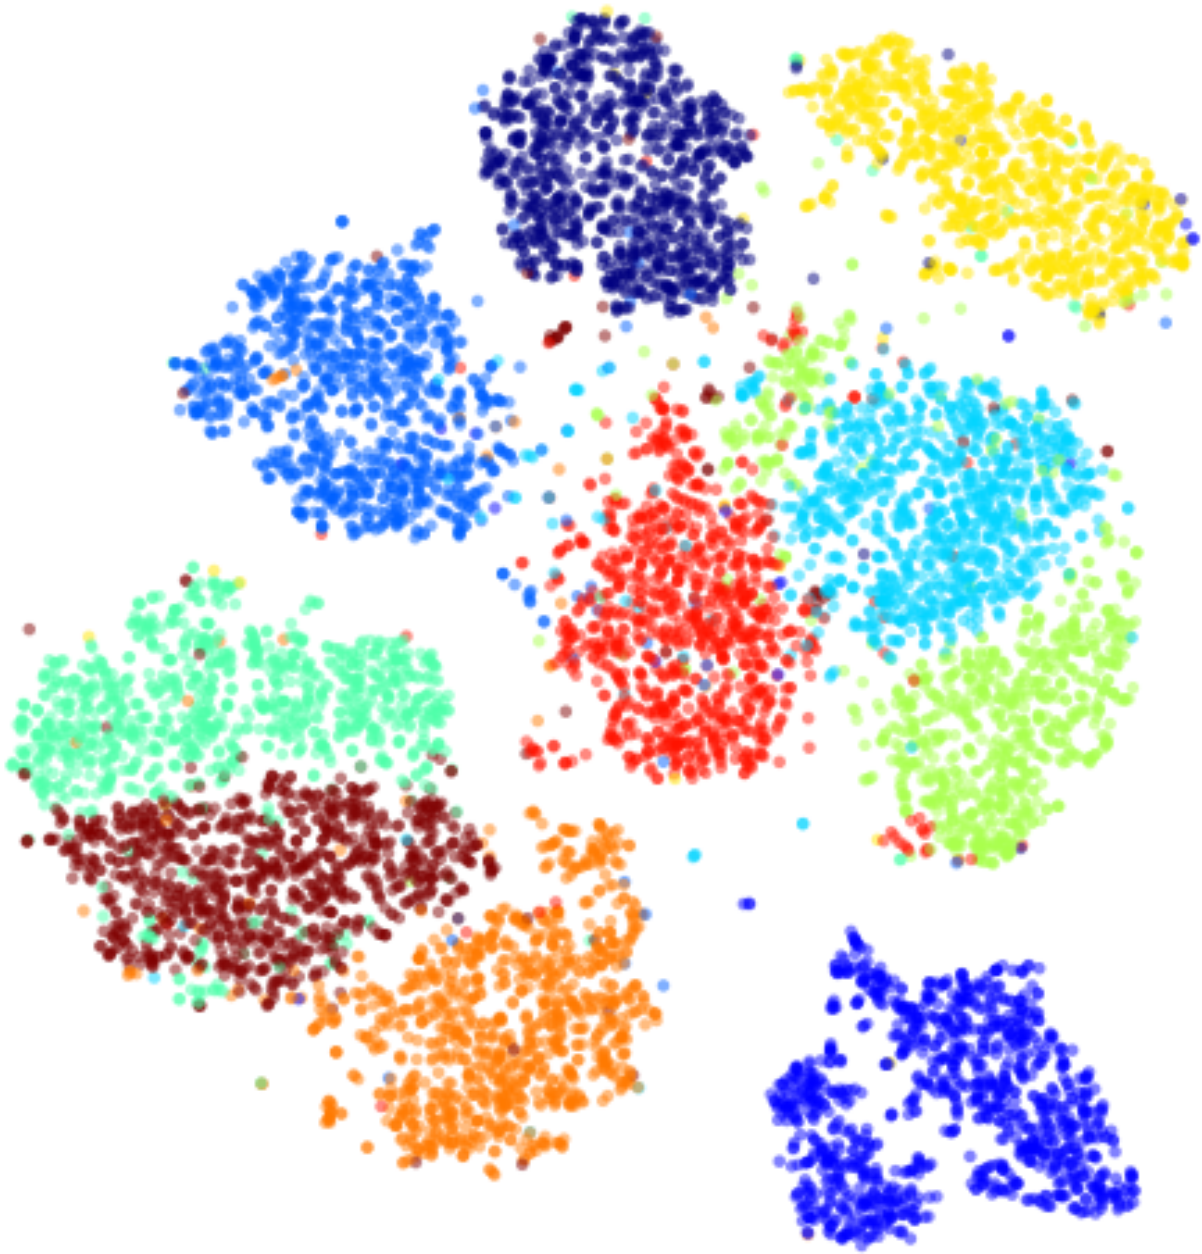
\includegraphics[width=\textwidth]{img/loracs/mnist/tsne/mnist2-tsne-vamp.png}
    \caption{Vam\p(500) prior}
\end{subfigure}
~
\begin{subfigure}[t]{0.3\textwidth}
    \centering
    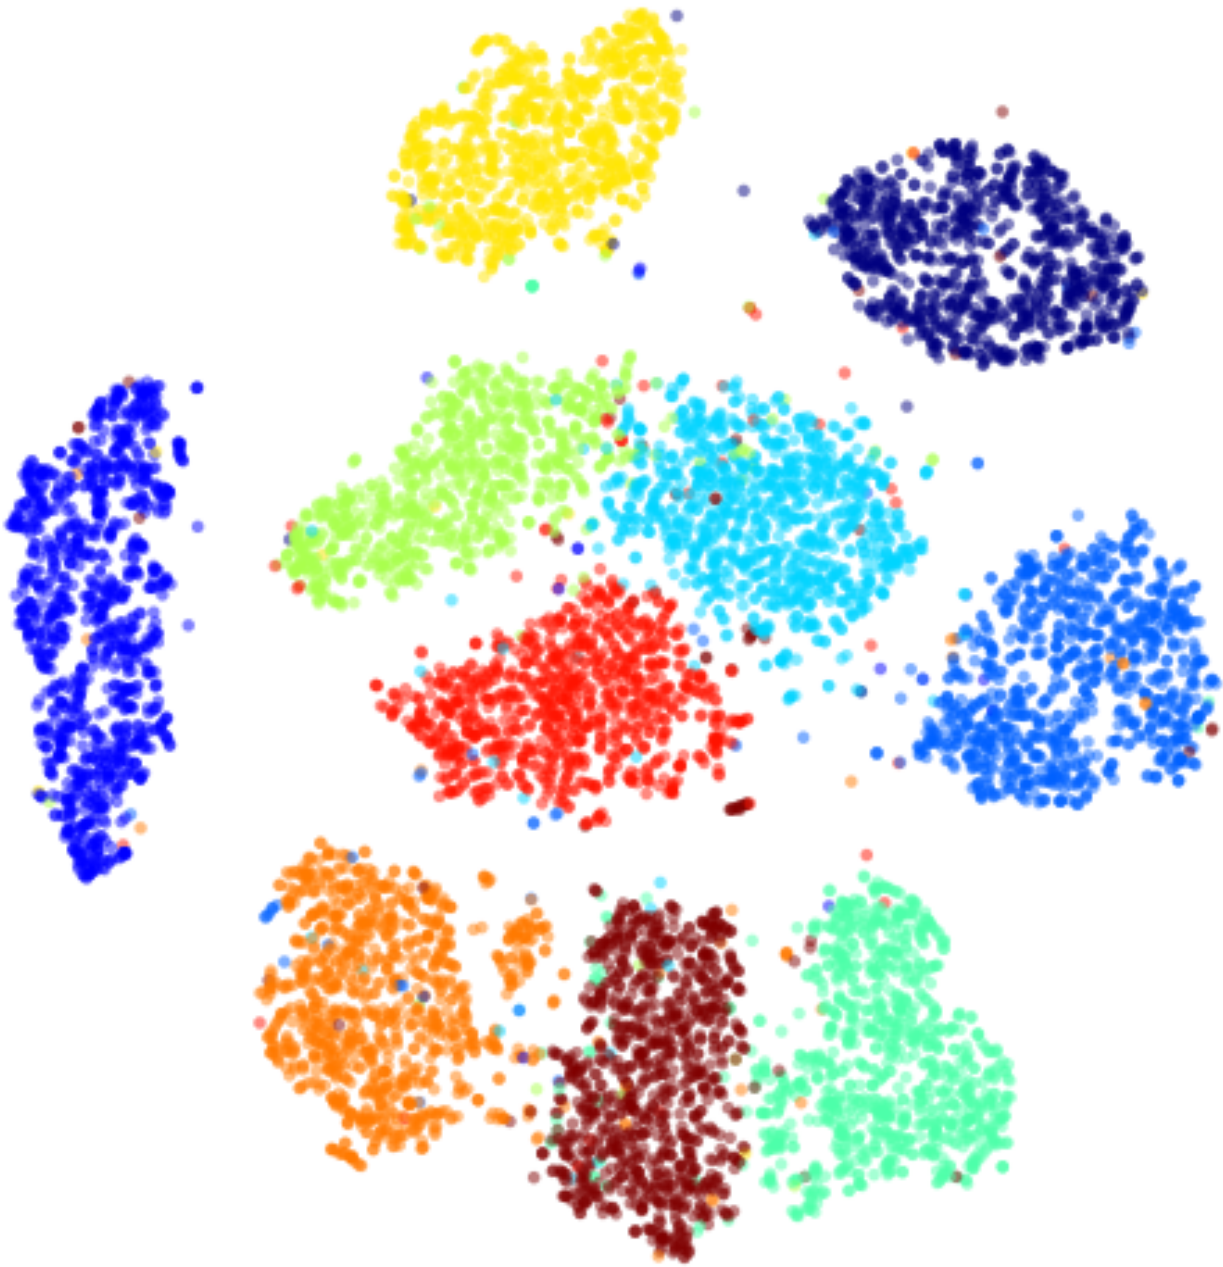
\includegraphics[width=\textwidth]{img/loracs/mnist/tsne/mnist2-tsne-maf.png}
    \caption{MAF prior}
\end{subfigure}
\begin{subfigure}[t]{0.3\textwidth}
    \centering
    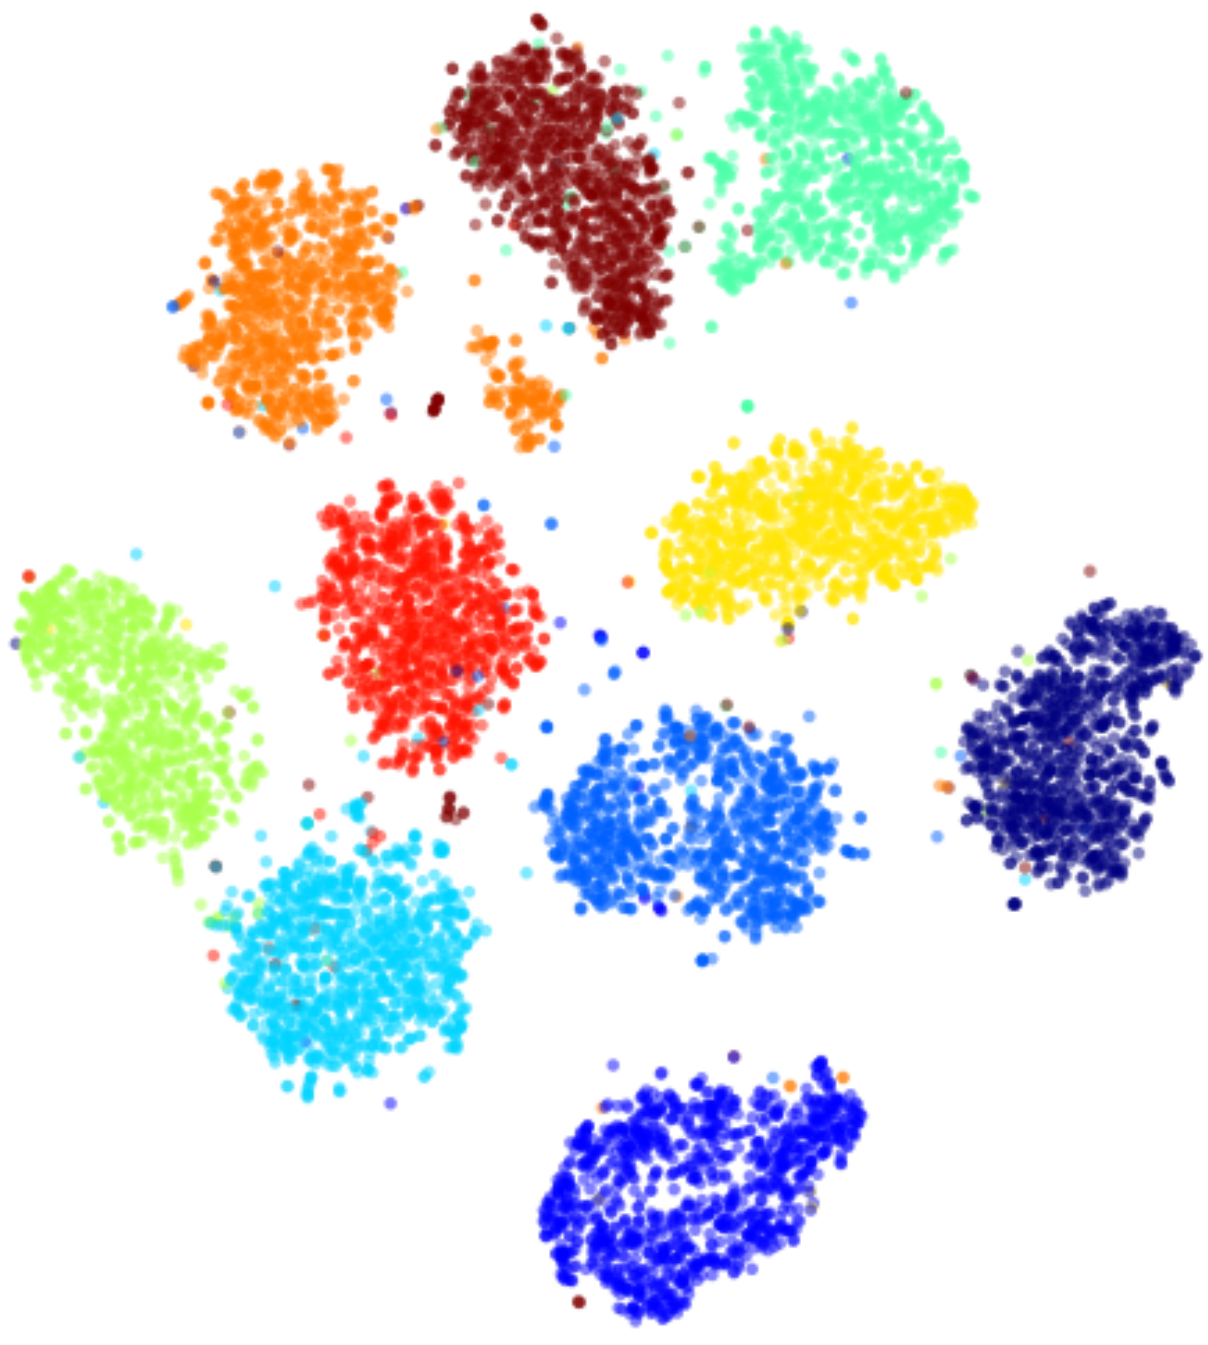
\includegraphics[width=\textwidth]{img/loracs/mnist/tsne/mnist2-tsne-tmc.png}
    \caption{\acronym(200) prior}
\end{subfigure}
\caption{TSNE visualizations of the latent space of the MNIST test set with various prior distributions, color-coded according to class.}
\label{fig:tsne}
\end{figure}

\begin{figure}[h]
    \centering
    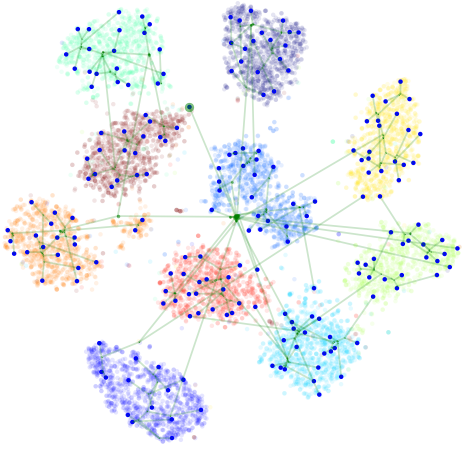
\includegraphics[width=0.5\textwidth]{img/loracs/mnist/tsne/mnist2-tsne-tmc-tree.png}
    \caption{A TSNE visualization of the latent space for the TMC(200) model with inducing points and one sample from $\q(\tree; \inducingpoints)$ plotted. Internal nodes are visualized by computing their expected posterior values, and branches are plotted in 2-d space.}
    \label{fig:mnist-tsne-tree}
\end{figure}


\begin{figure}[h]
\centering
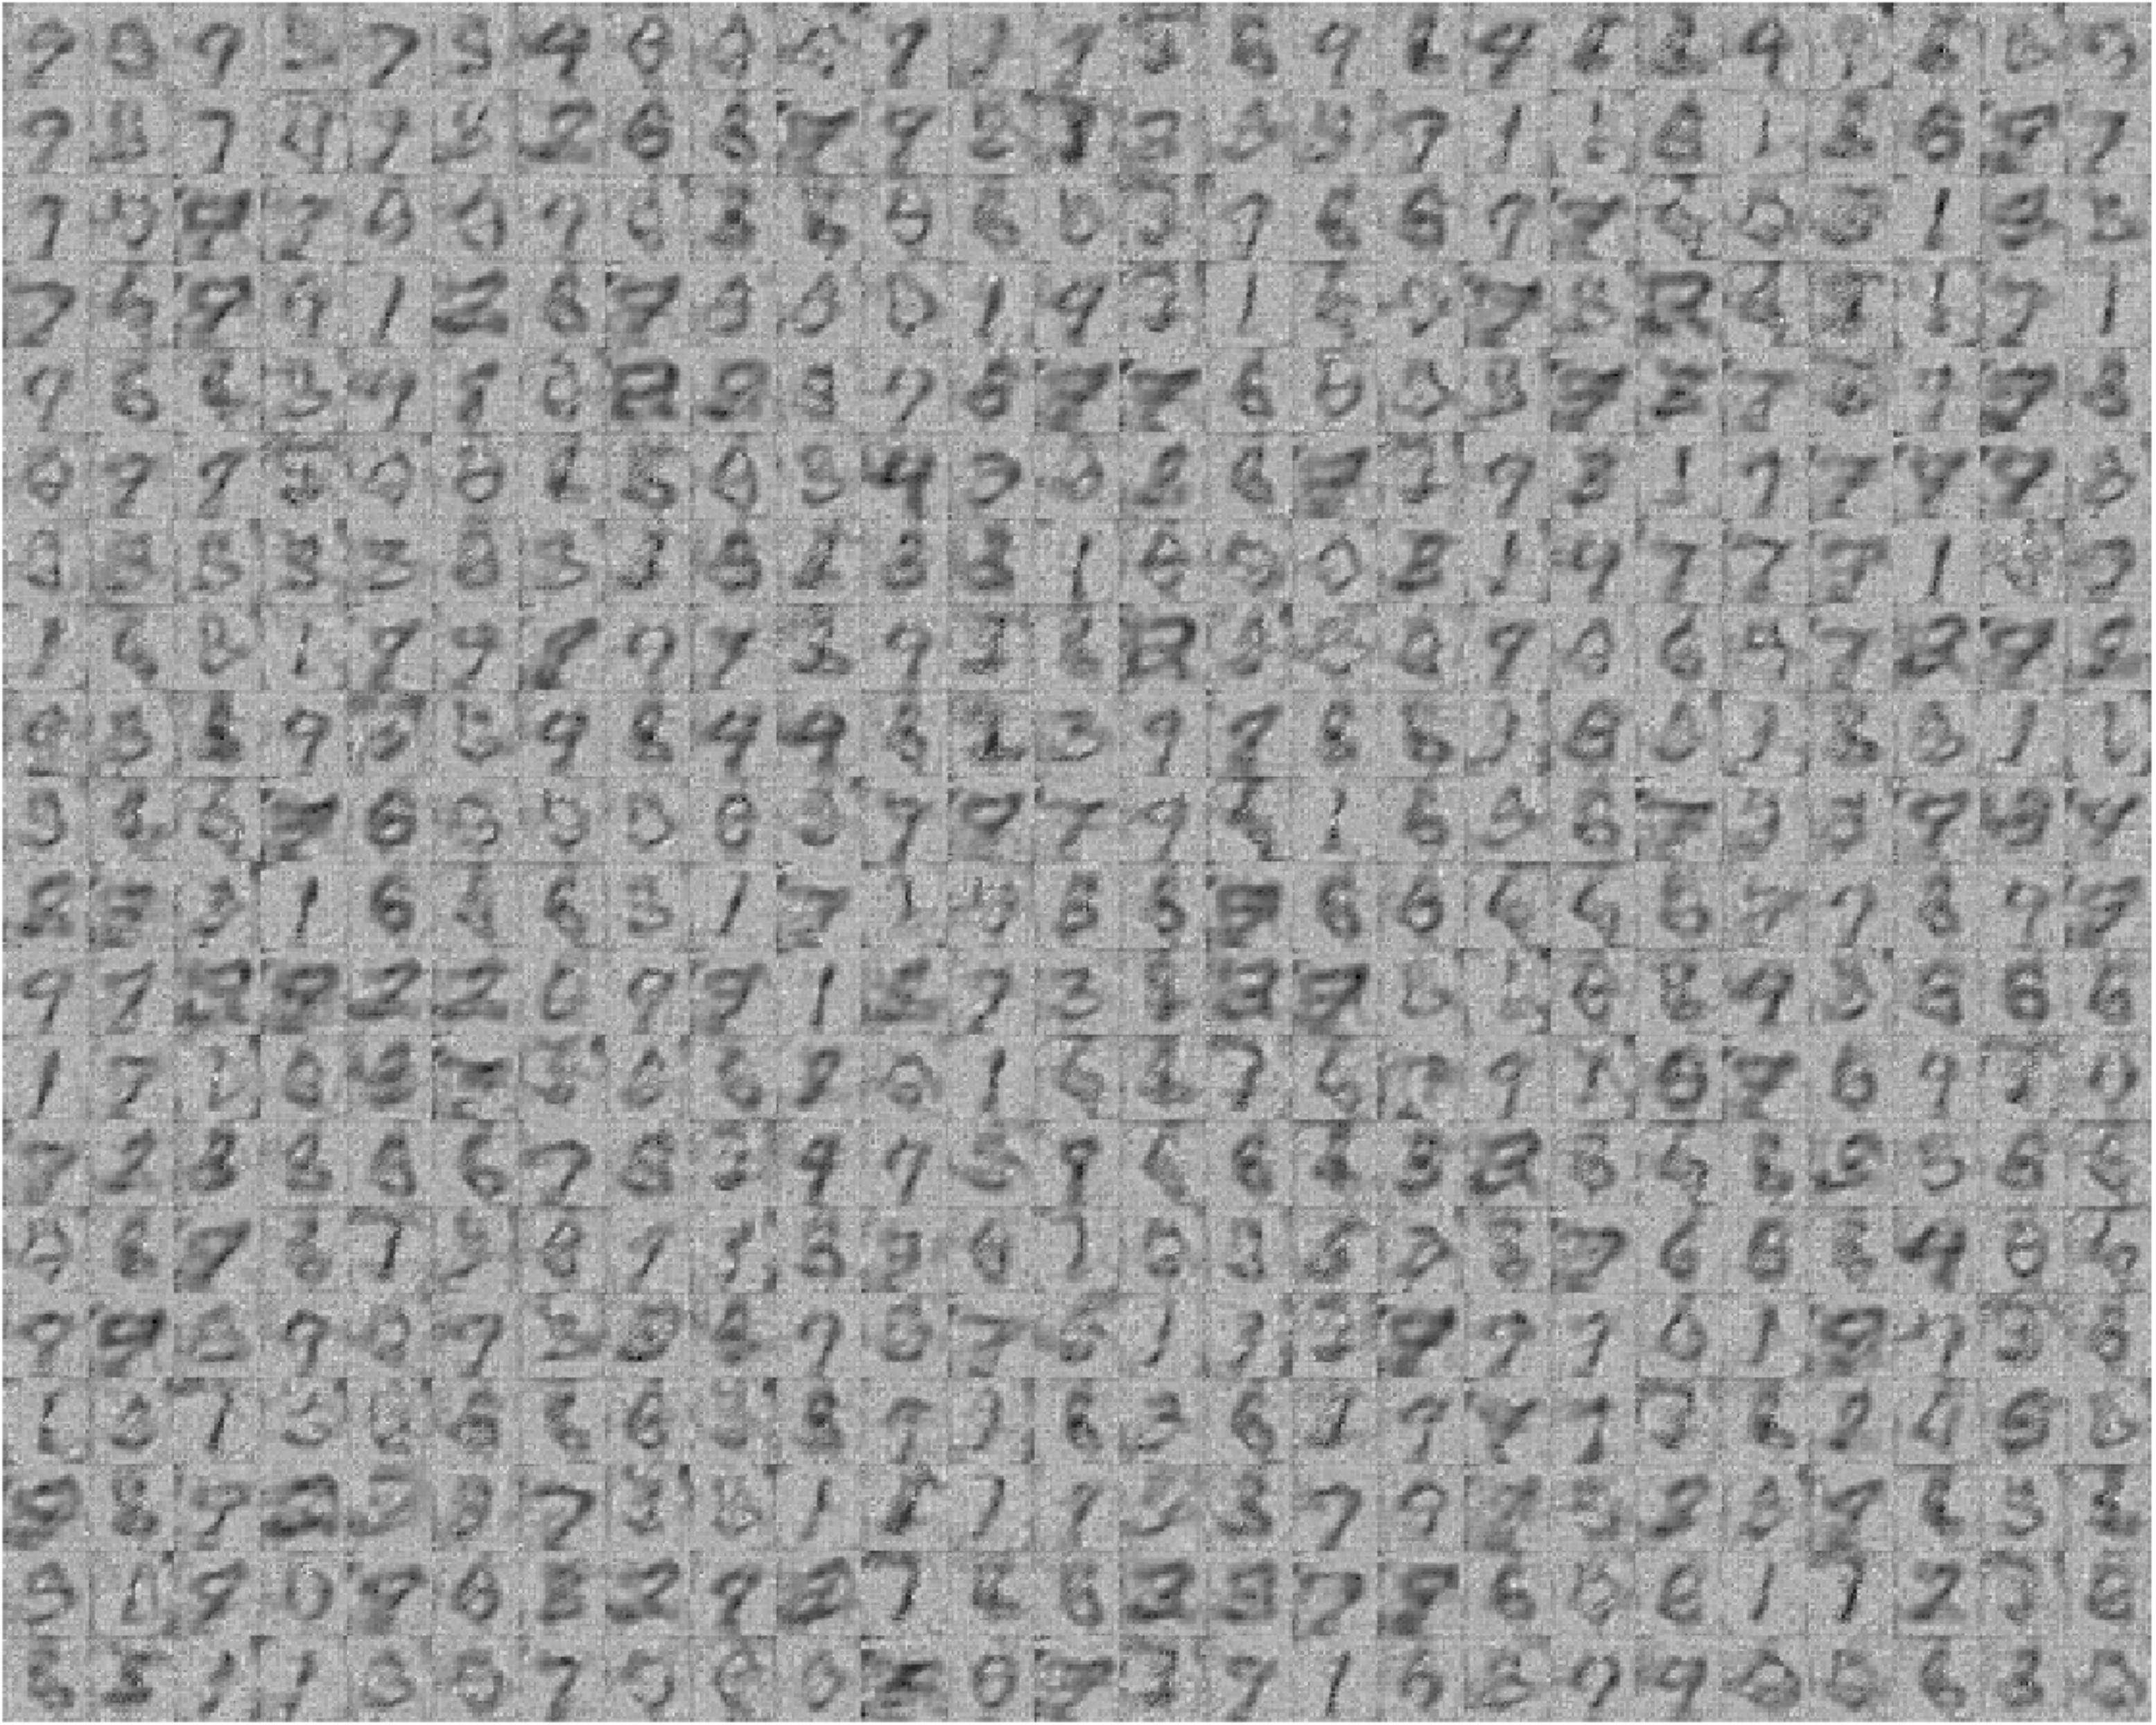
\includegraphics[width=0.5\textwidth]{img/loracs/mnist/mnist-vamp-inputs.png}
\caption{MNIST VampPrior learned pseudo-inputs.}
\label{fig:mnist-vamp-inducing}
\end{figure}
\begin{figure}[h]
\centering
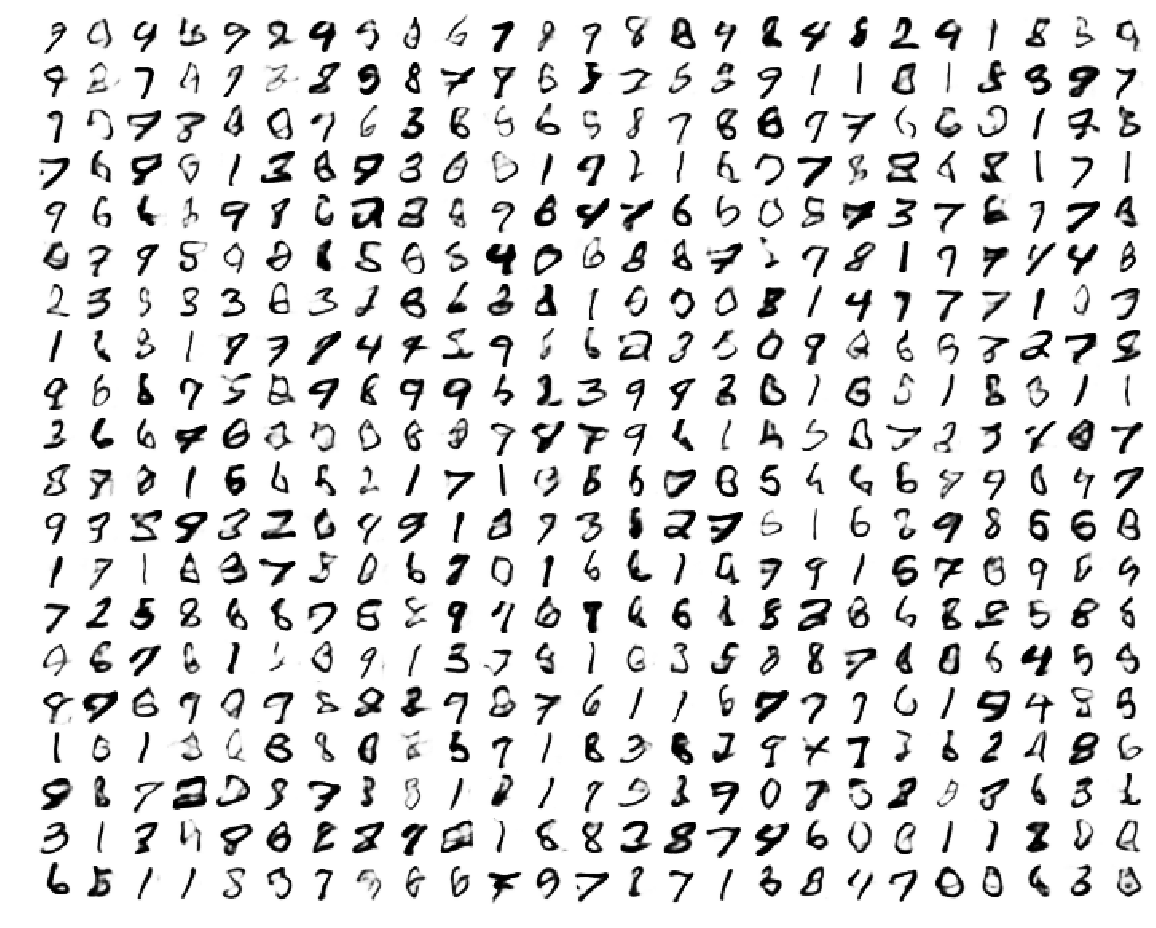
\includegraphics[width=0.5\textwidth]{img/loracs/mnist/mnist-vamp-outputs.png}
\caption{MNIST VampPrior reconstructed pseudo-inputs obtained by
deterministically encoding and decoding each pseudo-input.}
\label{fig:mnist-vamp-inducing-outputs}
\end{figure}

\begin{figure}[h]
\centering
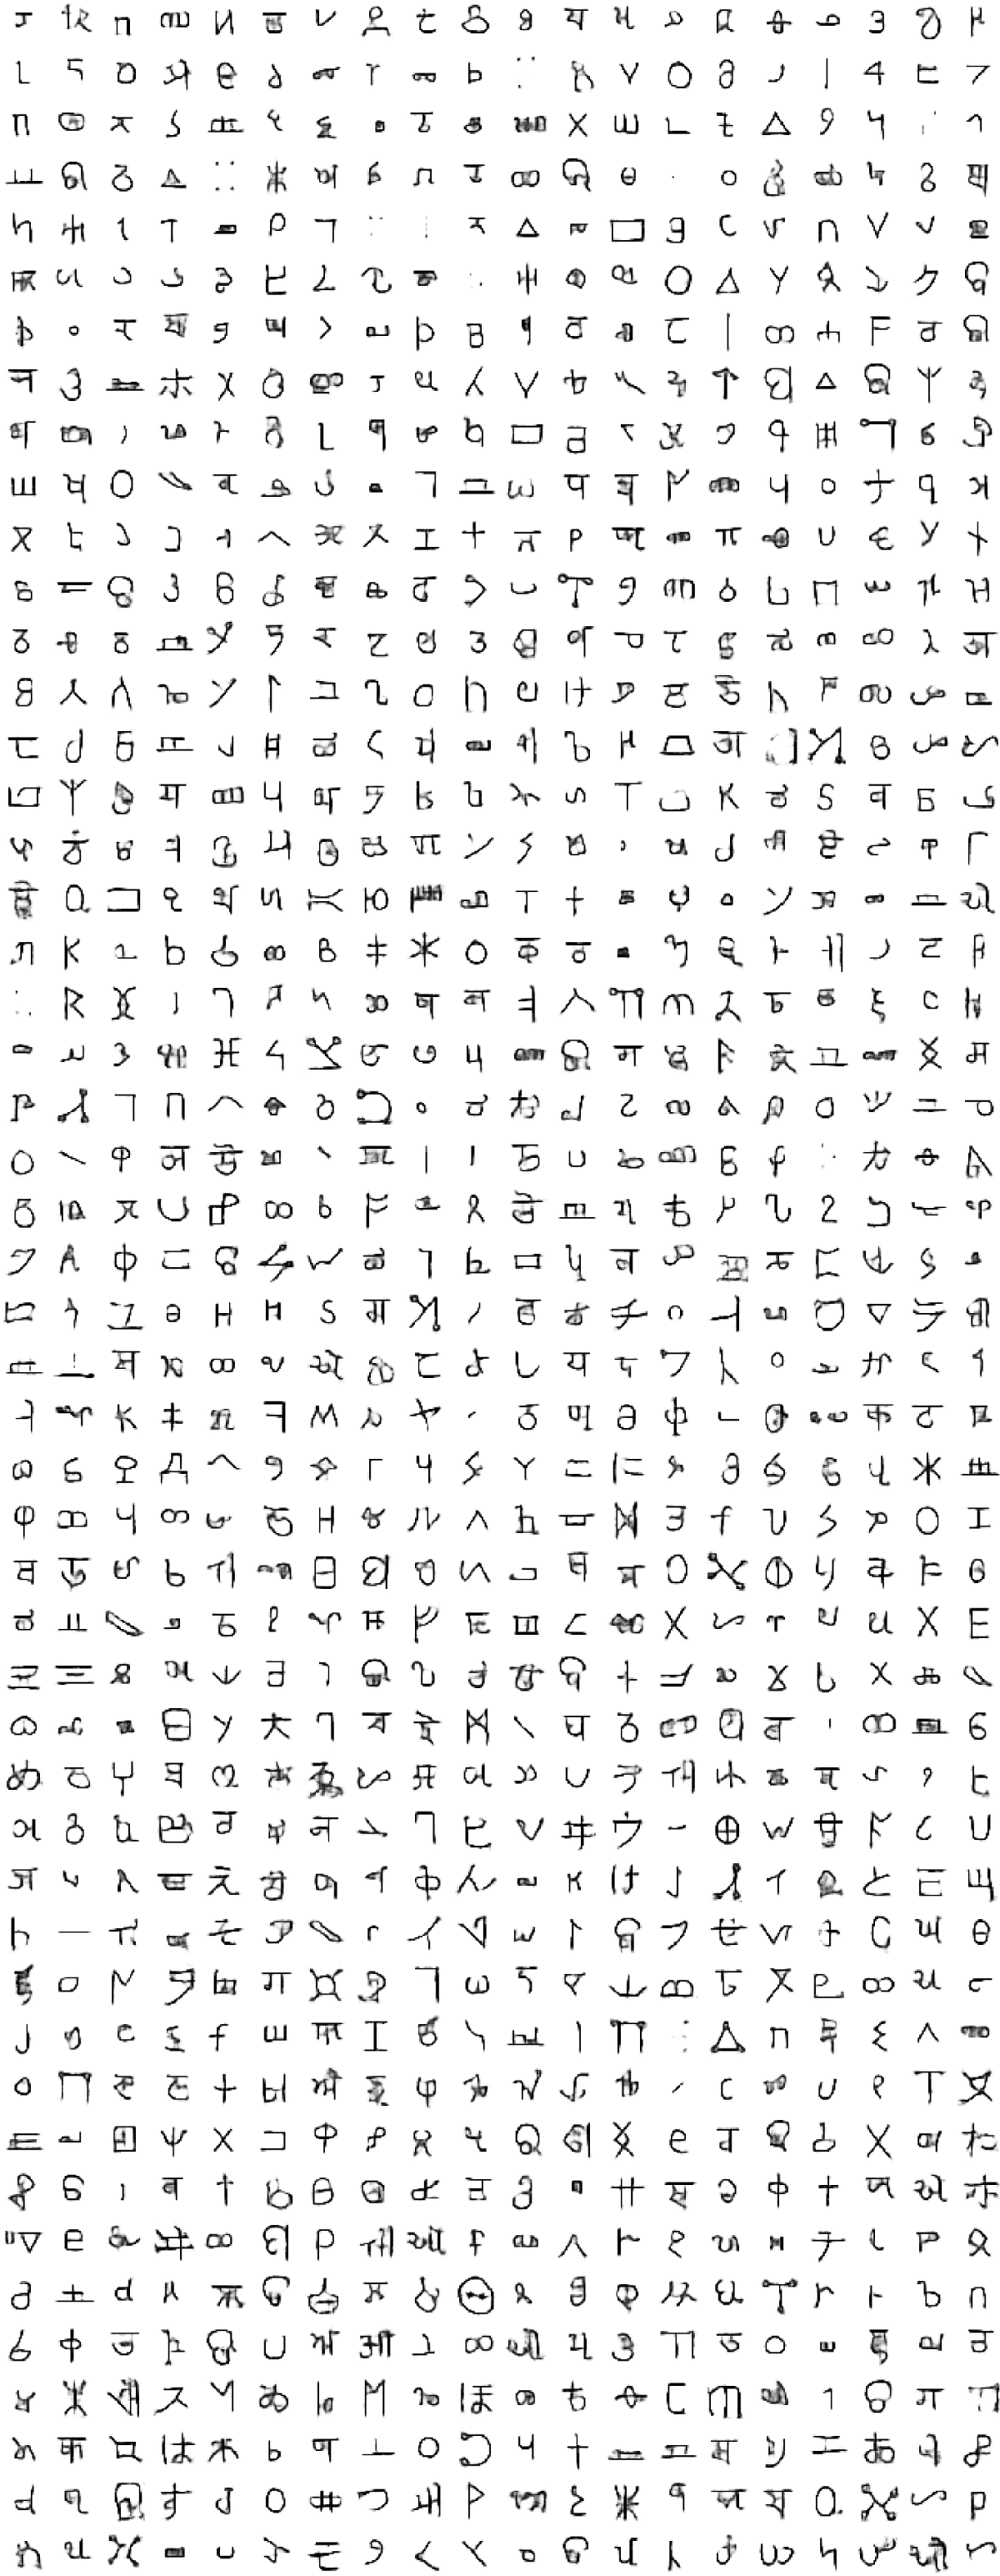
\includegraphics[width=0.4\textwidth]{img/loracs/omniglot/inducing-points.png}
\caption{Omniglot learned inducing points.}
\label{fig:omniglot-inducing-points}
\end{figure}

\begin{figure}[h]
\centering
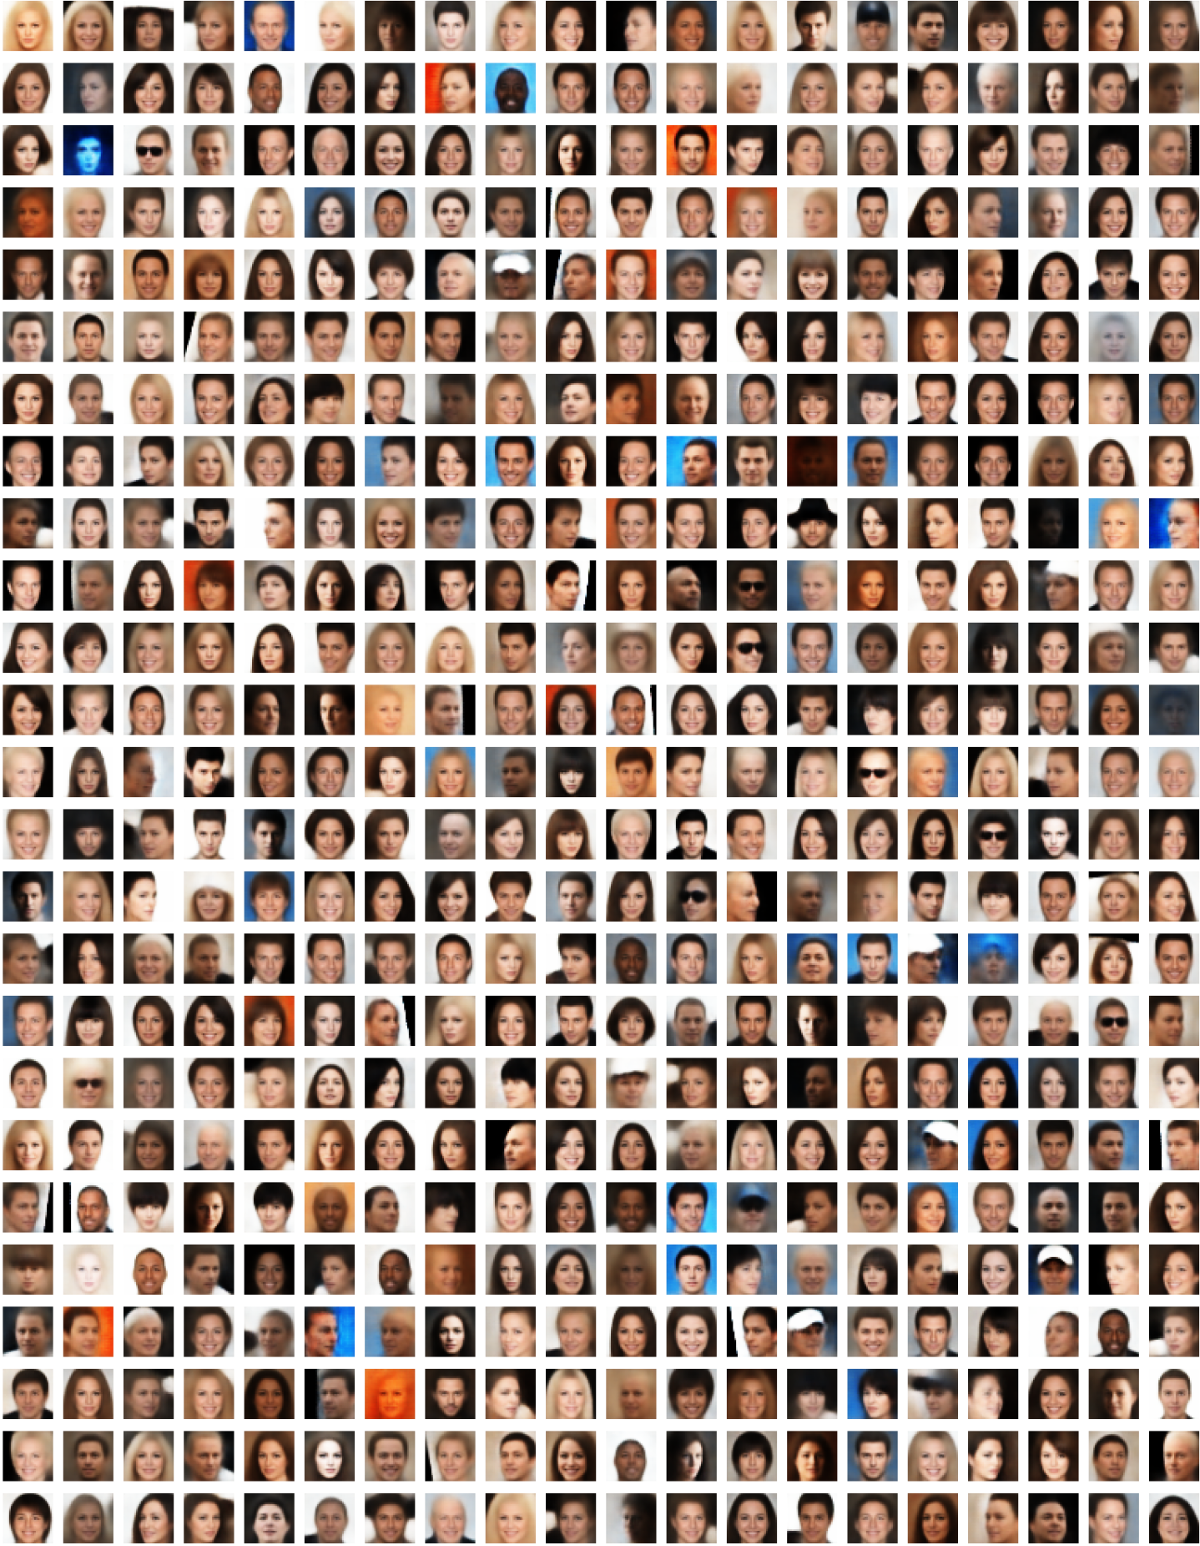
\includegraphics[width=0.8\textwidth]{img/loracs/celeba/inducing-points.png}
\caption{CelebA learned inducing points.}
\label{fig:celeba-inducing-points}
\end{figure}

\begin{landscape}
\section{Empirical results}
\thispagestyle{empty}

\begin{table}
\scriptsize
\centering
\setlength{\tabcolsep}{2pt}
\begin{tabular}{llllllllllll}
\hline
Labels per class             & 1                          & 10                         & 20                         & 30                         & 40                         & 50                         & 60                         & 70                         & 80                         & 90                         & 100                        \\ \hline
No prior                     & $0.506 \pm 0.095$          & $0.781 \pm 0.045$          & $0.820 \pm 0.023$          & $0.829 \pm 0.020$          & $0.836 \pm 0.026$          & $0.839 \pm 0.021$          & $0.844 \pm 0.017$          & $0.846 \pm 0.017$          & $0.847 \pm 0.015$          & $0.843 \pm 0.015$          & $0.848 \pm 0.014$          \\
Normal                       & $0.396 \pm 0.076$          & $0.775 \pm 0.051$          & $0.838 \pm 0.020$          & $0.861 \pm 0.016$          & $0.874 \pm 0.011$          & $0.883 \pm 0.011$          & $0.886 \pm 0.011$          & $0.892 \pm 0.010$          & $0.896 \pm 0.010$          & $0.899 \pm 0.011$          & $0.901 \pm 0.008$          \\
Vamp(500)                    & $0.539 \pm 0.094$          & $0.849 \pm 0.035$          & $0.891 \pm 0.019$          & $0.905 \pm 0.013$          & $0.911 \pm 0.016$          & $0.918 \pm 0.012$          & $0.921 \pm 0.009$          & $0.925 \pm 0.008$          & $0.929 \pm 0.007$          & $0.928 \pm 0.005$          & $0.932 \pm 0.005$          \\
DVAE\#                       & $0.453 \pm 0.101$          & $0.735 \pm 0.027$          & $0.784 \pm 0.017$          & $0.801 \pm 0.012$          & $0.813 \pm 0.013$          & $0.824 \pm 0.014$          & $0.830 \pm 0.012$          & $0.835 \pm 0.011$          & $0.841 \pm 0.007$          & $0.842 \pm 0.007$          & $0.846 \pm 0.008$          \\
MAF                          & $0.530 \pm 0.113$          & $0.869 \pm 0.029$          & $0.910 \pm 0.012$          & $0.923 \pm 0.012$          & $0.930 \pm 0.007$          & $0.933 \pm 0.010$          & $0.938 \pm 0.008$          & $0.940 \pm 0.008$          & $0.942 \pm 0.006$          & $0.944 \pm 0.006$          & $\mathbf{0.946 \pm 0.005}$ \\
\acronym(200) & $\mathbf{0.670 \pm 0.120}$ & $\mathbf{0.903 \pm 0.019}$ & $\mathbf{0.923 \pm 0.011}$ & $\mathbf{0.929 \pm 0.009}$ & $\mathbf{0.934 \pm 0.006}$ & $\mathbf{0.938 \pm 0.004}$ & $\mathbf{0.939 \pm 0.005}$ & $\mathbf{0.941 \pm 0.004}$ & $\mathbf{0.943 \pm 0.004}$ & $\mathbf{0.944 \pm 0.003}$ & $0.945 \pm 0.003$          \\ \hline
\end{tabular}
\caption{MNIST few-shot classification results.}
\label{tab:semisupervised-mnist}
\end{table}

\begin{table}
\scriptsize
\setlength{\tabcolsep}{2pt}
\centering
\begin{tabular}{llllll}
\toprule
Labels per class &                 1  &                 2  &                 5  &                 10 &                 15 \\
\midrule
No prior   &  $0.140 \pm 0.012$ &  $0.179 \pm 0.008$ &  $0.225 \pm 0.006$ &  $0.252 \pm 0.009$ &  $0.290 \pm 0.001$ \\
Normal     &  $0.107 \pm 0.007$ &  $0.134 \pm 0.010$ &  $0.187 \pm 0.008$ &  $0.246 \pm 0.006$ &  $0.285 \pm 0.000$ \\
Vamp(1000) &  $0.116 \pm 0.011$ &  $0.148 \pm 0.009$ &  $0.210 \pm 0.003$ &  $0.270 \pm 0.005$ &  $0.300 \pm 0.000$ \\
DVAE\#      &  $0.042 \pm 0.004$ &  $0.060 \pm 0.006$ &  $0.091 \pm 0.003$ &  $0.121 \pm 0.001$ &  $0.141 \pm 0.000$ \\
MAF        &  $0.096 \pm 0.008$ &  $0.129 \pm 0.006$ &  $0.177 \pm 0.010$ &  $0.222 \pm 0.007$ &  $0.237 \pm 0.002$ \\
\acronym(1000)  &  $\mathbf{0.173 \pm 0.005}$ &  $\mathbf{0.236 \pm 0.005}$ &  $\mathbf{0.330 \pm 0.008}$ &  $\mathbf{0.403 \pm 0.006}$ &  $\mathbf{0.441 \pm 0.000}$ \\
\bottomrule
\end{tabular}

\caption{Omniglot few-shot classification results.}
\label{tab:semisupervised-omniglot}
\end{table}
\begin{table}
\scriptsize
\setlength{\tabcolsep}{2pt}
\begin{tabular}{r|cc}
\toprule
     \# of inducing points &  200 & 500\\
\midrule
        & 0.9428 & 0.9474\\
\bottomrule
\end{tabular}
\centering
\caption{MNIST few-shot classification with labeled inducing points.}
\label{tab:inducing-point-labels}
\end{table}
\end{landscape}

\begin{figure}
\centering
\begin{subfigure}[h]{0.4\textwidth}
    \centering
    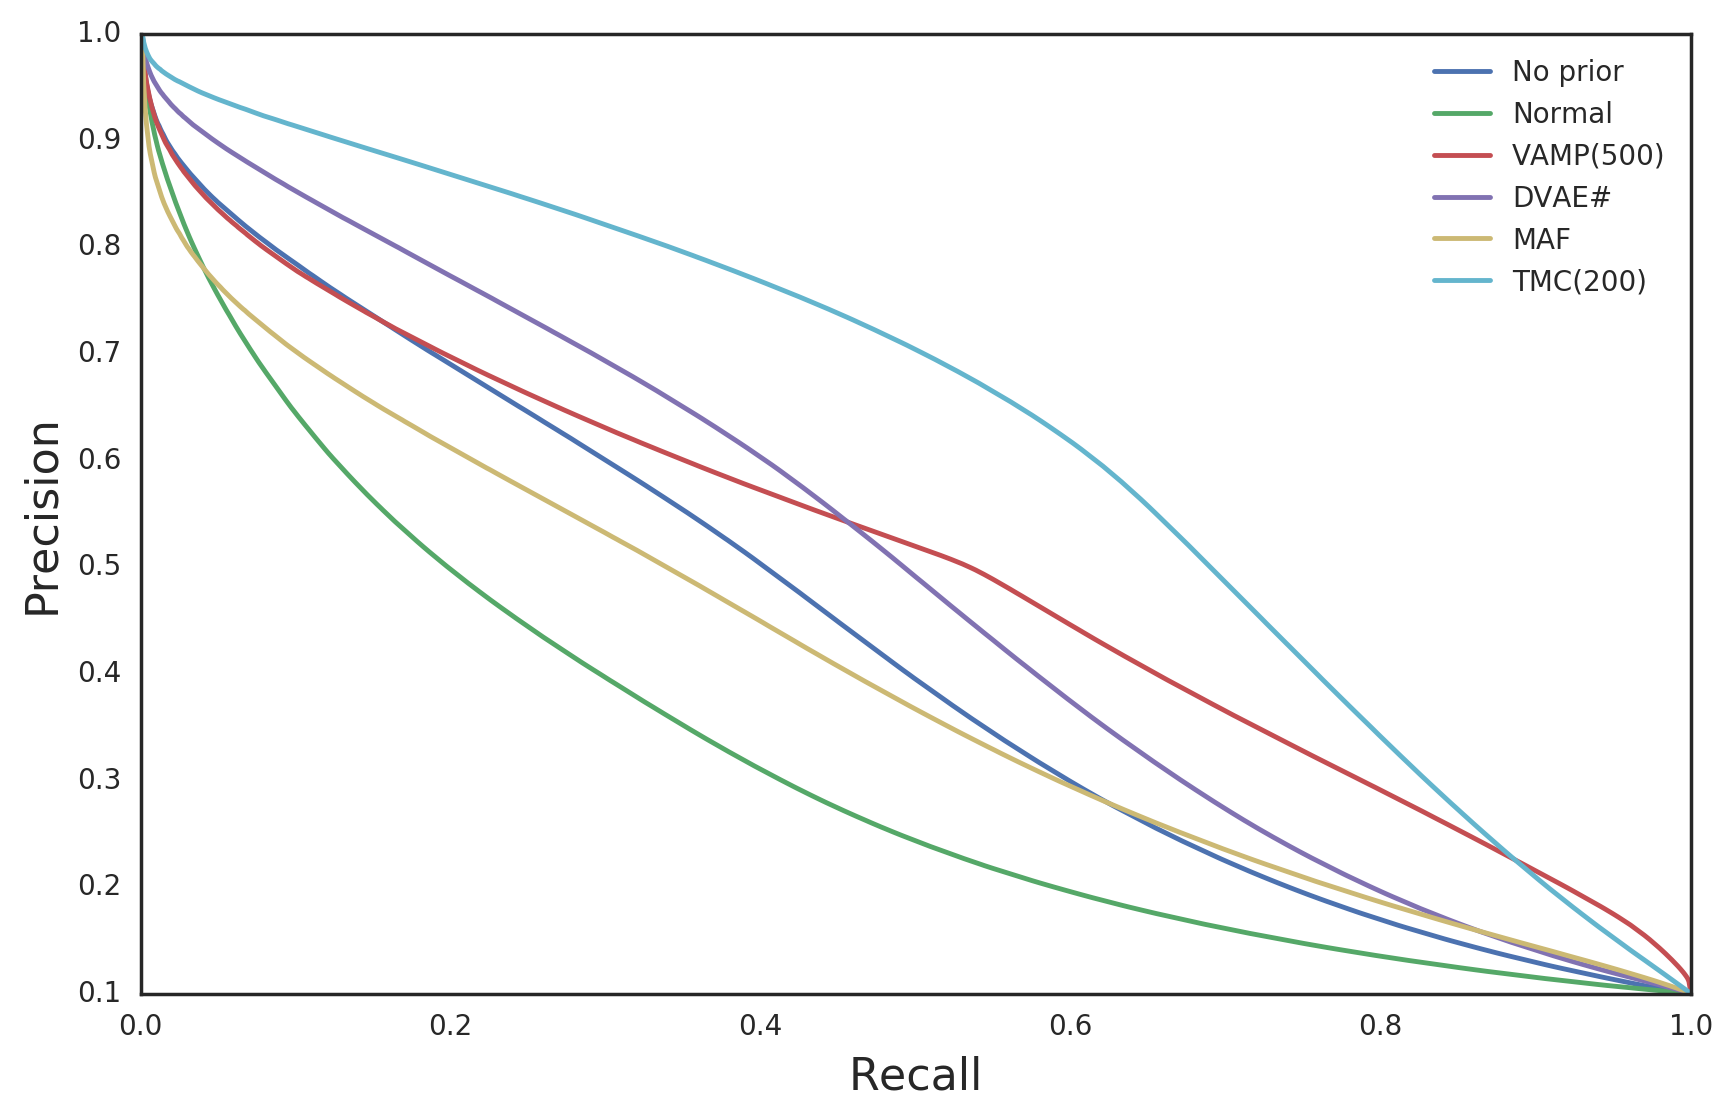
\includegraphics[width=\textwidth]{img/loracs/mnist/ir-mnist-joint.png}
    \caption{MNIST}
\end{subfigure}
\begin{subfigure}[h]{0.4\textwidth}
    \centering
    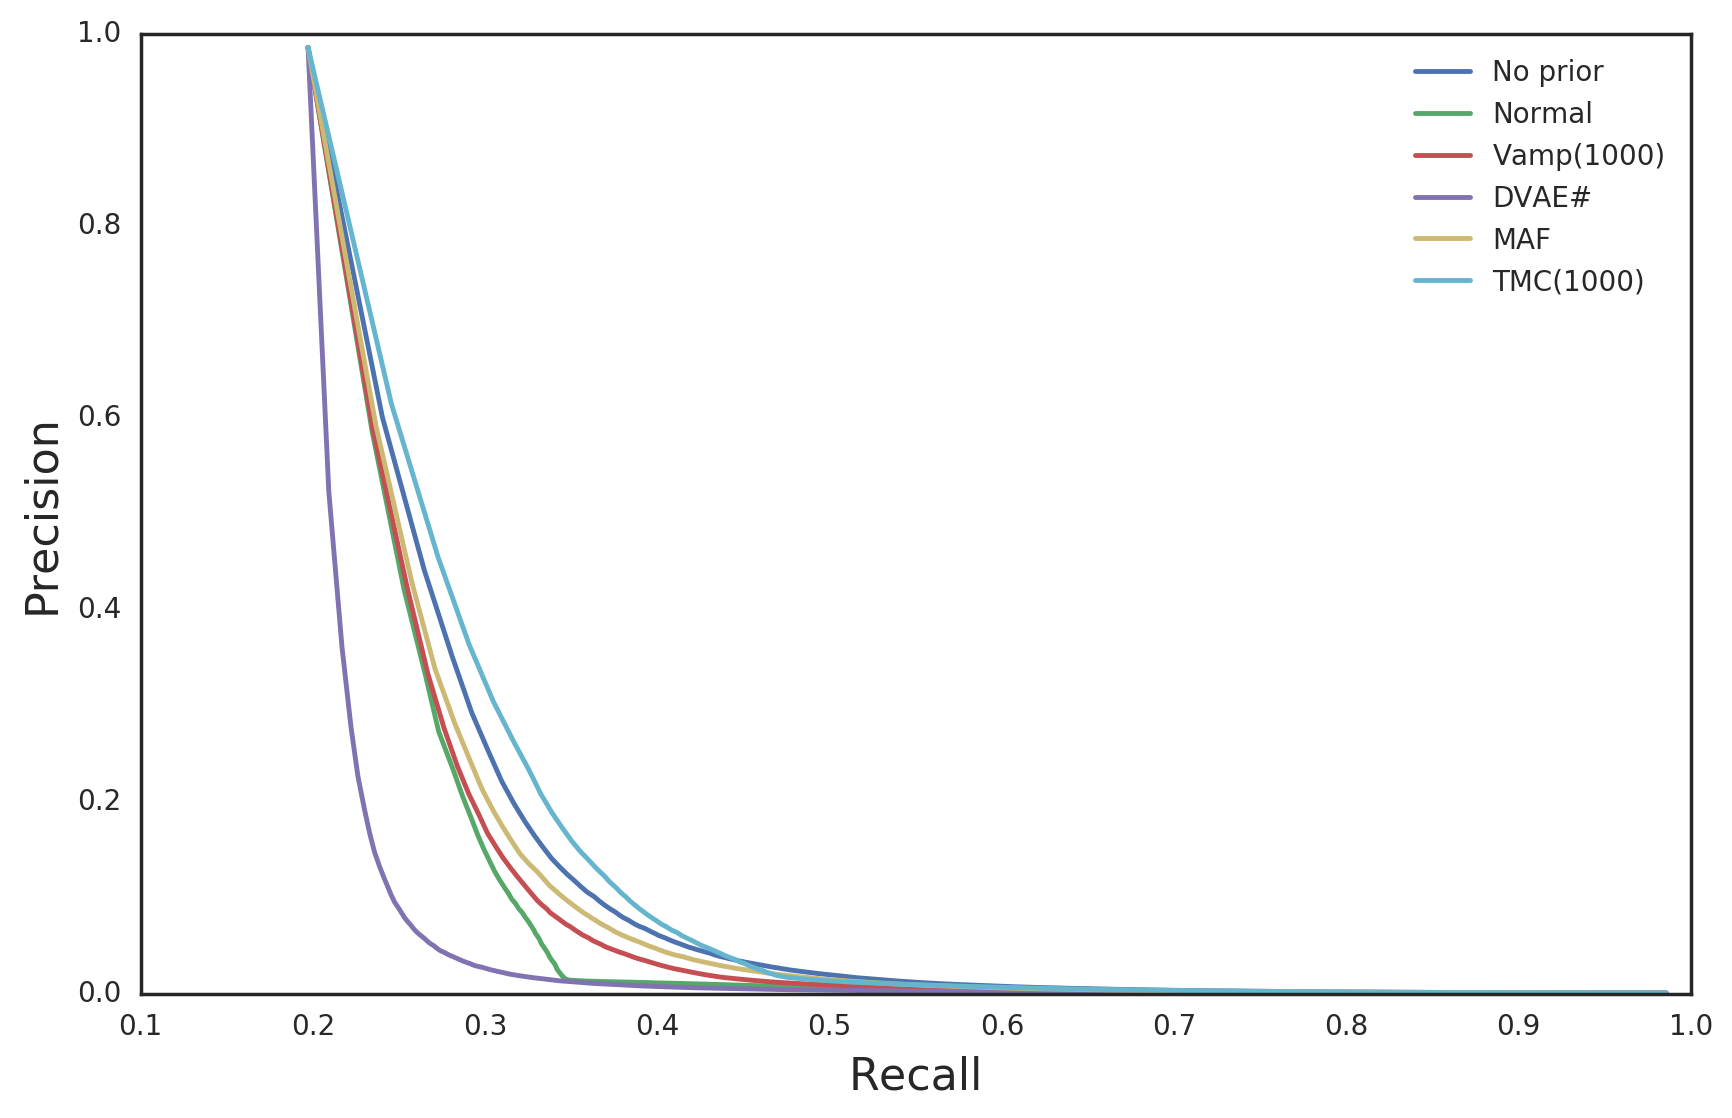
\includegraphics[width=\textwidth]{img/loracs/omniglot/ir-omniglot-joint.png}
    \caption{Omniglot}
\end{subfigure}
\caption{Averaged precision-recall curves over test datasets.}
\label{fig:prec-rec}
\end{figure}

\section{Algorithm details}
\label{sec:algorithm-details}

\subsection{Stick breaking process}
\label{sec:stick-breaking}
Consider inserting a node $\numdata + 1$ into the tree in between vertices $u$ and $v$
such that $t_v > t_u$,
creating branch $e_{\numdata + 1}$.
The inserted node has time $t_{\numdata + 1}$ with probability according to the stick breaking process, i.e.
\begin{equation}
\textstyle r(t_{\numdata+1}\given e_{\numdata+1}, V, E) =
\mathrm{Beta}\left(\frac{t_v - t_{\numdata + 1}}{1 - t_{\numdata + 1}}; a, b\right)\mathrm{Beta}\left(\frac{t_{\numdata + 1} - t_u}{1 - t_u}; a, b\right).
\end{equation}

\subsection{Belief propagation in TMCs}

The TMC is at the core of the \acronym\;
prior.
Recall that the TMC is
a prior over phylogenies $\tree$,
and after attaching a Gaussian random walk (GRW),
we obtain a distribution over $N$ vectors in $\mathbb{R}^d$,
corresponding to the leaves, $r(\latentdataset \given \tree)$.
However, the GRW samples
latent vectors at internal nodes $z_{V_{\text{int}}}$.
Rather than explicitly representing these values,
in this work we marginalize them out, i.e.
\begin{equation}
    r(\latentdataset \given \tree) = \int r(\latentdataset \given z_{V_{\text{int}}}, \tree)\p(z_{V_{\text{int}}} \given \tree) dz_{V_{\text{int}}}
\end{equation}
This marginalization process can be done efficiently, because our graphical model
is tree-shaped and all nodes have Gaussian likelihoods. Belief propagation is a message-passing
framework for marginalization and we utilize message-passing
for several TMC inference queries. The main queries we are interested in are:
\begin{enumerate}
    \item $r(\latentdataset, \tree)$ - for the purposes of MCMC, we are interested in computing the joint likelihood of a set of observed
    leaf values and a phylogeny.
    \item $r(\z_\n \given z_{\backslash n}, \tree)$ - this query computes the posterior density over one leaf given all the others;
    we use this distribution when computing the posterior predictive density of a TMC.
    \item $\nabla_{z_{\backslash n}} r(\z_\n \given z_{\backslash n}, \tree)$ - this query is the gradient of the predictive density 
    of a single leaf with respect to the values at all other leaves. This query is used
    when computing gradients of the ELBO w.r.t $\inducingpoints$ in the \acronym\;prior.
\end{enumerate}

\paragraph{Message passing} Message
passing treats the tree as an undirected graph. 
We first pick start node $v_{\text{start}}$
and request messages from each of $v_{\text{start}}$'s neighbors.

Message passing is thereafter defined recursively. 
When a node $v$ has requested messages from a source node $s$,
it thereafter requests messages from all its neighbors but $s$.
The base case for this recursion is a leaf node $v_\n$,
which returns a message with the following contents:
\begin{equation}
    \nu_\n = \bm{0};\quad \mu_\n = \z_\n;\quad \log \z_\n = 0;\quad \nabla_{\nu_\n}(\nu) = \bm{1};\quad \nabla_{\nu_\n}(\mu) = \bm{0};\quad \nabla_{\mu_\n}(\mu) = \bm{1}
\end{equation}
where bold numbers $\bm{0}\triangleq (0,\ldots,0)^\top$ and $\bm{1}\triangleq (1,\ldots,1)^\top$ denote vectors obtained by repeating a scalar $d$ times.

In the recursive case, consider being at a node $i$ and receiving a set of messages from its neighbors $M$.
\begin{equation}
\begin{split}
    \nu_i = \frac{1}{\sum_{m \in M}\frac{1}{\nu_m + e_{im}}} ;\quad \mu_i = v_i \sum_{m \in M} \frac{\mu_m}{\nu_m + e_{im}}\\
\end{split}
\end{equation}
where $e_{im}$ is the length of the edge between nodes $i$ and $m$.
These messages are identical to those used in \citet{Boyles2012}.

Additionally, our messages include gradients w.r.t. \emph{every} leaf node
downstream of the message.
We update each of these gradients when computing the new message
and pass them along to the source node.
Gradients with respect to one of these nodes $j$ are calculated as
\begin{equation}
\begin{split}
    \nabla_{\nu_j}(\nu) &= \nabla_{\nu_j} \nu_i\\
    \nabla_{\nu_j}(\mu) &= \nabla_{\nu_j} \mu_i\\
    \nabla_{\mu_j}(\mu) &= \nabla_{\mu_j} \mu_i\\
\end{split}
\end{equation}
The most complicated message is the $\log Z_i$ message, which depends
on the number of incoming messages. $v_{\text{start}}$ gets
three incoming messages,
all other nodes get only two. Consider
two messages from nodes $v_k$ and $v_l$:
\begin{equation}
\begin{split}
    \Sigma_i &\triangleq (\nu_k + e_{ik} + \nu_l + e_{il})I \\
    \log Z_i &= -\frac{1}{2}\|\mu_k - \mu_l\|^2_{\Sigma_i} - \frac{1}{2}\left(\log|\Sigma_i| _ d\log2\pi\right)
\end{split}
\end{equation}
For three messages from nodes
$v_k$, $v_l$, and $v_m$:
\begin{equation}
\begin{split}
    \Sigma_i &\triangleq \left((\nu_k + e_{ik})(\nu_l + e_{il}) + (\nu_l + e_{il})(\nu_m + e_{im}) + (\nu_m + e_{im})(\nu_k + e_{ik})\right)I \\
    \log Z_i &= -\frac{1}{2}\left((\nu_m + e_{im})\|\mu_k - \mu_l\|^2_{\Sigma_i} + (\nu_k + e_{ik})\|\mu_l - \mu_m\|^2_{\Sigma_i} + (\nu_l + e_{il})\|\mu_m - \mu_k\|^2_{\Sigma_i}\right) - \frac{1}{2}\log|\Sigma_i| - \log2\pi
\end{split}
\end{equation}

With these messages, we can answer all the aforementioned inference queries.
\begin{enumerate}
    \item We can begin message passing at any internal node and compute: $\log r(\latentdataset, \tree) = \sum_{v \in V} \log Z_v$
    \item We start message passing at $v_\n$. $r(\z_\n \given z_{\backslash n}, \tree)$ is a Gaussian with mean $\mu_\n$ and variance $\nu_\n$.
    \item $\nabla_{z_{\backslash n}} r(\z_\n \given z_{\backslash n}, \tree)$ is $\nabla_{z_{\backslash n}} \N(\z_\n \given \mu_\n, \nu_\n I)$,
    which in turn utilizes gradients sent via message passing.
\end{enumerate}

\paragraph{Implementation} We chose
to implement the TMC and message
passing in Cython because we found raw Python to be
too slow due to function call and type-checking
overhead. Furthermore, we used diagonal rather than
scalar variances in the message passing implementation
to later support diagonal variances handed 
from the variational posterior over $\z_\n$.

\subsection{Variational inference for the \acronym\;prior}
\label{sec:inference-details}

The \acronym\; prior involves first sampling a tree
from the posterior distribution over TMCs
with $\inducingpoints$ as leaves.
We then sample a branch and time
for each data $\z_\n$ according
to the posterior predictive
distribution described in \autoref{sec:bnhc}.
We then sample a $\z_\n$ from
the distribution induced by the GRW likelihood model.
Finally, we pass the sampled $\z_\n$
through the decoder.
\begin{equation}
    \begin{split}
        \tree &\sim \p(\tree ; \inducingpoints) \\
        e_\n, t_\n &\sim \p(e_\n, t_\n | \tree) \\
        \z_\n | e_\n, t_\n, \tree &\sim \p(\z_\n | e_\n, t_\n, \tree; \inducingpoints) \triangleq r(s_{M + 1} = \z_\n | e_\n, t_\n, \tree) \\
        \x_\n | \z_\n &\sim \p_\genparam(\x_\n | \z_\n)
    \end{split}
\end{equation}

Consider sampling the optimal $q^*(\tree; \inducingpoints)$.

\begin{equation}
\begin{split}
    q^*(\tree; \inducingpoints) 
    &\propto \exp{\E_\q\left[\log \p(\tree, \latentdataset, \dataset)\right]} \\
    &\propto \exp{\log \p(\tree ; \inducingpoints) + \sum_\n \E_\q\left[\p(\z_\n | e_\n, t_\n, \tree)\right]} \\
    &\propto \exp{\log \mathrm{TMC}_\n(\tree; a, b) + \sum_{m = 1}^M \log r(\inducingpoint_m | \inducingpoint_{1:m - 1}, \tree) \\&+ \sum_\n \E_\q\left[\log \p(\z_\n | e_\n, t_\n, \tree)\right]} \\
\end{split}
\end{equation}
We  set $\q(\tree; \inducingpoints) = r(\tree \given \inducingpoints)$.
We use additional variational factors
$\q(e_\n)$,
$q_{\xi}(t_\n | e_\n, \z_\n; \inducingpoints)$,
and
$q_\recparam(\z_\n | \x_\n)$.
$q_{\xi}(t_\n | e_\n, \z_\n; \inducingpoints)$ is a
recognition network that outputs
the attach time for a particular branch.
Since the $\q(\tree; \inducingpoints)$ and $\p(\tree; \inducingpoints)$ terms
cancel out, we obtain the following ELBO.
\begin{equation}
    \begin{split}
    \L[q] &\triangleq \E_\q \left[\log \frac{\prod_\n \p(e_\n, t_\n | \tree) \p(\z_\n | e_\n, t_\n, \tree; \inducingpoints)\p_\genparam(\x_\n | \z_\n)}{\prod_\n \q(e_\n)q_{\xi}(t_\n | e_\n, \z_\n; \inducingpoints)q_\recparam(\z_\n | \x_\n)}\right] \\
    \end{split}
\end{equation}

\paragraph{Inference procedure}
In general, $\q(\tree; \inducingpoints)$ can
be sampled using vanilla SPR Metropolis-Hastings,
so samples from this distribution are readily available. 

For each data in the minibatch $\x_\n$, we pass it
through the encoder to obtain $\q(\z_\n | \x_\n)$.
We then compute
\begin{equation}
    q^*(e_\n) = \exp{\E_\q\left[\log \p(e_\n | t_\n, \z_\n, \tree; \inducingpoints)\right]}
\end{equation}
This quantity is computed by looping
over every branch $b$ of 
a sample from $\q(\tree)$,
storing incoming messages at each node,
passing the $\mu$ and $\nu$
and a sample from $\q(\z_\n | \x_\n)$
into $q_\xi(t_\n | e_\n, \inducingpoints, \z_\n)$,
outputting a logistic-normal distribution
over times for that branch. We sample that
logistic normal to obtain a time $t$
to go with branch $b$. We can then compute
the log-likelihood of $\z_\n$ if it were
to attach to $b$ and $t$, using TMC
inference query \#2.
This log-likelihood is added to the TMC prior log-probability
of the branch being selected to obtain
a joint probability $\E_\q\left[\log \p(e_\n)\p(t_\n)\p(\z_\n | e_\n, t_\n, \tree; \inducingpoints)\right]$ over the branch.
After doing this for every branch, we normalize
the joint likelihoods to obtain
the optimal categorical distribution over every branch
for $\z_\n$, $q^*(e_\n)$. We then sample this
distribution to obtain an attach location and time
$e_\n, t_\n$ for each data in the minibatch.

The next stage is to compute gradients w.r.t. to the
learnable parameters of the model ($\genparam$, $\inducingpoints$, $\recparam$, and $\xi$).
In the process of calculating $q^*(e_\n)$,
we have obtained samples from its corresponding 
$q_\xi(t_\n | e_\n, \z_\n, \tree; \inducingpoints)$ and $\q(\z_\n | \x_\n)$.
We plug these into the ELBO and can compute
gradients via automatic differentiation w.r.t. $\recparam$,
$\genparam$, and $\xi$. Computing gradients w.r.t.
$\inducingpoints$ is more tricky. We first examine the ELBO.

\begin{equation}
    \L[\q] = \E_\q \left[\log \frac{\prod_\n \p(e_\n|\tree) \p(t_\n) \p(\z_\n | e_\n, t_\n, \tree; \inducingpoints)\p_\genparam(\x_\n | \z_\n)}{\prod_\n \q(e_\n)\q_{\xi}(t_\n | e_\n, \z_\n; \inducingpoints)q_\recparam(\z_\n | \x_\n)}\right]
\end{equation}

Consider the gradient of the ELBO with respect to $\inducingpoints$.

\begin{equation}
    \begin{split}
    \nabla_{\inducingpoints}\L[q] &=
    \nabla_{\inducingpoints}\E_\q \left[\log \frac{\prod_\n \p(e_\n|\tree) \p(t_\n) \p(\z_\n | e_\n, t_\n, \tree; \inducingpoints)\p_\genparam(\x_\n | \z_\n)}{\prod_\n \q(e_\n)q_{\xi}(t_\n | e_\n, \z_\n; \inducingpoints)q_\recparam(\z_\n | \x_\n)}\right] \\
    &= \nabla_{\inducingpoints}\sum_{\tree} \q(\tree; \inducingpoints)\E_\q \left[\log \frac{\prod_\n \p(e_\n|\tree) \p(t_\n) \p(\z_\n | e_\n, t_\n, \tree; \inducingpoints)\p_\genparam(\x_\n | \z_\n)}{\prod_\n \q(e_\n)q_{\xi}(t_\n | e_\n, \z_\n; \inducingpoints)q_\recparam(\z_\n | \x_\n)}\right]\\
    &= \sum_\tree \q(\tree; \inducingpoints)\nabla_{\inducingpoints}\E_\q\left[\log \frac{\prod_\n \p(e_\n|\tree) \p(t_\n) \p(\z_\n | e_\n, t_\n, \tree; \inducingpoints)\p_\genparam(\x_\n | \z_\n)}{\prod_\n \q(e_\n)q_{\xi}(t_\n | e_\n, \z_\n; \inducingpoints)q_\recparam(\z_\n | \x_\n)}\right]\\
    &+ \sum_\tree \left(\nabla_{\inducingpoints} \q(\tree; \inducingpoints)\right)\E_\q \left[\log \frac{\prod_\n \p(e_\n|\tree) \p(t_\n) \p(\z_\n | e_\n, t_\n, \tree; \inducingpoints)\p_\genparam(\x_\n | \z_\n)}{\prod_\n \q(e_\n)q_{\xi}(t_\n | e_\n, \z_\n; \inducingpoints)q_\recparam(\z_\n | \x_\n)}\right]\\
    &= \sum_\tree \q(\tree; \inducingpoints)\nabla_{\inducingpoints}\E_\q\left[\log \frac{\prod_\n \p(e_\n|\tree) \p(t_\n) \p(\z_\n | e_\n, t_\n, \tree; \inducingpoints)\p_\genparam(\x_\n | \z_\n)}{\prod_\n \q(e_\n)q_{\xi}(t_\n | e_\n, \z_\n; \inducingpoints)q_\recparam(\z_\n | \x_\n)}\right]\\
    &+ \sum_\tree \left(\q(\tree;\inducingpoints)\nabla_{\inducingpoints} \log \q(\tree; \inducingpoints)\right)\E_\q \left[\log \frac{\prod_\n \p(e_\n|\tree) \p(t_\n) \p(\z_\n | e_\n, t_\n, \tree; \inducingpoints)\p_\genparam(\x_\n | \z_\n)}{\prod_\n \q(e_\n)q_{\xi}(t_\n | e_\n, \z_\n; \inducingpoints)q_\recparam(\z_\n | \x_\n)}\right]\\
    &= \E_{\q(\tree)}\left[\nabla_{\inducingpoints}\E_\q\left[\log \frac{\prod_\n \p(e_\n|\tree) \p(t_\n) \p(\z_\n | e_\n, t_\n, \tree; \inducingpoints)\p_\genparam(\x_\n | \z_\n)}{\prod_\n \q(e_\n)q_{\xi}(t_\n | e_\n, \z_\n; \inducingpoints)q_\recparam(\z_\n | \x_\n)}\right]\right.\\
    &+ \left.\nabla_{\inducingpoints} \log \q(\tree; \inducingpoints)\E_\q \left[\log \frac{\prod_\n \p(e_\n|\tree) \p(t_\n) \p(\z_\n | e_\n, t_\n, \tree; \inducingpoints)\p_\genparam(\x_\n | \z_\n)}{\prod_\n \q(e_\n)q_{\xi}(t_\n | e_\n, \z_\n; \inducingpoints)q_\recparam(\z_\n | \x_\n)}\right]\right]\\
    &= \E_{q}\left[
        \nabla_{\inducingpoints}\left(-\log \q(e_\n) - \log \q(t_\n \given \z_\n, e_\n, \tree; \inducingpoints) + \log \p(\z_\n \given e_\n, t_\n, \tree; \inducingpoints)\right)
    \right] \\
    &+ \E_\q\left[\nabla_{\inducingpoints}\left(\log \q(\tree) + \log \q(e_\n)\right)\log\frac{\p(e_\n | \tree)}{\q(e_\n)}\frac{\p(\z_\n \given \z_\n, e_\n, t_\n, \tree; \inducingpoints)}{\q(t_\n \given \z_\n, e_\n, \tree; \inducingpoints)}\right]
    \end{split}
\end{equation}

In the last step, we expand out expectation over $e_\n$ and
then pass the derivative through like we did for $\tree$.
The gradients w.r.t. $\q(e_\n)$ are zero, since $q^*(e_\n)$ is
a partial optimum of the ELBO and we are left with:.
\begin{equation}
    \begin{split}
        \nabla_{\inducingpoints}\L[q] &= \E_\q\left[\nabla_{\inducingpoints}\log \p(\z_\n | e_\n, t_\n, \tree; \inducingpoints)\right] - \E_\q\left[\log \q(t_\n \given \z_\n, e_\n, \tree; \inducingpoints)\right] \\
        &+ \E_\q\left[\nabla_{\inducingpoints} \log \q(\tree; \inducingpoints)\log\frac{\p(e_\n | \tree)}{\q(e_\n)}\frac{\p(\z_\n \given \z_\n, e_\n, t_\n, \tree; \inducingpoints)}{\q(t_\n \given \z_\n, e_\n, \tree; \inducingpoints)}\right]
    \end{split}
\end{equation}
The first term of the gradient is the expected gradient
of the posterior predictive density w.r.t $\inducingpoints$.
This can be calculated by using TMC inference query \#3
using samples from $\q(e_\n)$ and $\q(t_\n \given \z_\n, e_\n, \tree; \inducingpoints)$. The second term also uses the same gradients, by means
of the chain rule to differentiate through the time-amortization network.
The third term of this gradient is a score function gradient,
which we decide to not use due to the high-variance nature of score function gradients. We found that we were able to obtain strong results even with biased gradients.

\section{Details of experiments}
\label{sec:implementation-details}

We implemented the \acronym\;prior in Tensorflow
and Cython. 
For MNIST and Omniglot, our architectures are in \autoref{tab:mnist-arch} and CelebA is in \autoref{tab:celeba-arch}.

\begin{table}
\centering
\begin{subfigure}[h]{0.4\textwidth}
\begin{tabular}{lll}
\toprule
Layer type & Shape \\
\midrule
Conv + ReLU & [3, 3, 64], stride 2 \\
Conv + ReLU & [3, 3, 32], stride 1 \\
Conv + ReLU & [3, 3, 16], stride 2 \\
FC + ReLU & 512 \\
Gaussian & 40 \\
\bottomrule
\end{tabular}
\caption{Encoder}
\end{subfigure}
\begin{subfigure}[h]{0.4\textwidth}
\begin{tabular}{lll}
\toprule
Layer type & Shape \\
\midrule
FC + ReLU & 3136 \\
Deconv + ReLU & [3, 3, 32], stride 2 \\
Deconv + ReLU & [3, 3, 32], stride 1 \\
Deconv + ReLU & [3, 3, 1], stride 2 \\
Bernoulli & \\
\bottomrule
\end{tabular}
\caption{Decoder}
\end{subfigure}
\caption{Network architectures for MNIST and Omniglot}
\label{tab:mnist-arch}
\end{table}

\begin{table}
\centering
\begin{subfigure}[h]{0.4\textwidth}
\begin{tabular}{lll}
\toprule
Layer type & Shape \\
\midrule
Conv + ReLU & [3, 3, 64], stride 2 \\
Conv + ReLU & [3, 3, 32], stride 1 \\
Conv + ReLU & [3, 3, 16], stride 2 \\
FC + ReLU & 512 \\
Gaussian & 40 \\
\bottomrule
\end{tabular}
\caption{Encoder}
\end{subfigure}
\begin{subfigure}[h]{0.4\textwidth}
\begin{tabular}{lll}
\toprule
Layer type & Shape \\
\midrule
FC + ReLU & 4096 \\
Deconv + ReLU & [3, 3, 32], stride 2 \\
Deconv + ReLU & [3, 3, 32], stride 1 \\
Deconv + ReLU & [3, 3, 3], stride 2 \\
Bernoulli & \\
\bottomrule
\end{tabular}
\caption{Decoder}
\end{subfigure}
\caption{Network architectures for CelebA}
\label{tab:celeba-arch}
\end{table}

In general, we trained the model interleaving
one gradient step with 100 sampling steps for $\q(\tree; \inducingpoints)$.
We also found that experimenting with values of $a$ and $b$
in the TMC prior did not impact results significantly.
We initialized the networks with weights
from a VAE trained for 100 epochs and inducing points
were initialized using k-means. All parameters
were trained using Adam \citep{Kingma2014adam} with a $10^{-3}$ learning rate
for an 100 epochs with learning rate decay to $10^{-5}$ for the last 20 epochs. 
Finally, we initialized trees with all node times close to 0,
to emulate a VAE prior.

\subsection{Baseline details}
All baselines were trained with the default architecture.
They were trained for 400 epochs,
with KL warmup ($\beta$ started at $10^{-2}$, and ramped up to $\beta = 1$
linearly over 50 epochs). They were trained using Adam with a
learning rate of $10^{-3}$, with a learning rate of $10^{-5}$ for
the last 80 epochs.

DVAE\# was trained using the default implementation from
\url{https://github.com/QuadrantAI/dvae}, which is hierarchical
VAE consisting of two Bernoulli latent variables, 200-dimensional each.
Each is learned via a feed-forward neural network 4-layers deep.
The default DVAE\# implementation also uses statically binarized MNIST
where we use dynamically binarized.
